\documentclass[assignment03_Solutions]{subfiles}

%\IfSubStr{\jobname}{\detokenize{Solutions}}{\toggletrue{solutions}}{\toggletrue{solutions}}

\IfSubStr{\jobname}{\detokenize{Solutions}}{\toggletrue{solutions}}{\togglefalse{solutions}}

\fancypagestyle{firstpage}

{\rhead{Assignment 3 \linebreak \textit{Version: \today}}}

\title{Assignment 3: Classification, Logistic Regression, and Gradient Descent}
\author{Machine Learning}
\date{Fall 2019}

\begin{document}

\maketitle
\thispagestyle{firstpage}


\begin{learningobjectives}
\bi
\item Learn about the framing of the classification problem in machine learning.
\item Learn about the logistic regression algorithm.
\item Learn about gradient descent for optimization.
\ei
\end{learningobjectives}

\begin{priorknowledge}
\bi
\item Supervised learning problem framing.
\item Training / testing splits.
\ei
\end{priorknowledge}
\vspace{1em}

%
%\begin{recall}[Supervised Learning Problem Setup]
%We are given a training set, $(\mlvec{x_1}, y_1), (\mlvec{x}_2, y_2), \ldots, (\mlvec{x}_n, y_n)$ where each $\mlvec{x_i}$ represents an element of an input space (e.g., a d-dimensional feature vector) and each $y_i$ represents an element of an output space (e.g., a scalar target value).  Our goal is to determine a function $\hat{f}$ that maps from the input space to the output space.
%
%We assume there is a loss function, $\ell$, that determines the amount of loss that a particular prediction $\hat{y}_i$ incurs due to a mismatch with the actual output $y_i$.  The best possible model, $\hat{f}^\star$, is the one that minimizes these losses over the training set.  This notion can be expressed with the following equation.
%\begin{align}
%\hat{f}^\star &= \argmin_{\hat{f}} \sum_{i=1}^n \ell \left ( \hat{f}(\mlvec{x_i}), y_i \right )
%\end{align} 
%\end{recall}


\section{The Classification Problem}

So far in this class we've looked at supervised learning problems where the responses $y_i$ are continuous-valued and the loss function is quadratic ($\ell(y, \hat{y}) = (y-\hat{y})^2$).  This is an example of a regression problem.  There are many times, however, where it is unnatural to frame a problem as a regression.  For instance, it may be the case that $y_i$ does not come from a continuous range but instead can only take on a few different values.  This sort of problem is known as a classification problem.  For instance, you might want to have a system that takes in an image of a person and predicts their identity.  The identity could be thought of as the output, $y_i$, and it would only make sense for $y_i$ to be one of several values (e.g., each value might represent a particular person the system was trained to recognize).  In this assignment you'll learn about a special case of the classification problem known as binary classification (where $y_i$ is either 0 or 1, e.g., a Paul versus Sam recognizer).

In this assignment we will formalize the binary classification problem and see a very useful algorithm for solving it called \emph{logistic regression}.  You will also see that the logistic regression algorithm is a very natural extension of linear regression.  Our plan for getting there is going to be pretty similar to what we did for linear regression.
\bi
\item Build some mathematical foundations
\item Introduce logistic regression from a top-down perspective
\item Learn about logistic regression from a bottom-up perspective
\ei

\section{Formalizing the Classification Problem}
Let's start by making the binary classification problem more formal.  Suppose, we are given a training set, $(\mlvec{x_1}, y_1), (\mlvec{x_2}, y_2), \ldots, (\mlvec{x_n}, y_n)$, where each $\mlvec{x_i}$ is an element of the input space (e.g., a vector) and each $y_i$ is a binary number (either 1 or 0).  In this setting we will attempt to use the training data to determine a function, $\hat{f}^\star$, that predicts the corresponding output, $y$, for any possible input, $\mathbf{x}$.  For example,  $\mathbf{x}$ could be an image and $y_i$ could be $1$ when the picture contains a puppy and $0$ otherwise.

\vspace{1em}
\begin{exercise}[(10 minutes)]
\bes
\item Given this partial setup of the binary classification problem, we still need to specify the loss function, $\ell$.  Recall that $\ell$ takes as input the actual output $y$, and the predicted output $\hat{y}$.  What function could you use for $\ell$ that would result in the learning algorithm choosing a good model?  If the choice of $\ell$ depends on the application, how so?

\begin{boxedsolution}
An easy choice is to output a $1$ if the values don't match and a $0$ otherwise (essentially counting the number of mistakes the model makes).  Alternatively, you could have different penalties for a false positive (the model says $\hat{y} = 1$, but the actual value is $y = 0$) or false negatives (the model says $\hat{y} = 0$, but the actual value is $y = 1$). 
\end{boxedsolution}

\item \label{ex:minmistakes}
One natural choice for $\ell$, which you may have already come up with, is to define our loss function as $\ell(y, \hat{y}) = \mathbb{I}[y \neq \hat{y}]$ (the funny looking $\mathbb{I}$ is the indicator function that takes on value 1 when the condition inside is true and 0 otherwise.  Given this choice the supervised learning problem becomes:
\begin{align}
\hat{f}^\star &= \argmin_{\hat{f}} \sum_{i=1}^n \mathbb{I} \left [  \hat{f}(\mlvec{x_i}) \neq y_i\right ] \enspace . \label{eq:minimizeerror}
\end{align}

Convert Equation~\ref{eq:minimizeerror} to English to make sure you understand it.
\begin{boxedsolution}
The equation says that $\hat{f}^\star$ is the function that minimizes the number of mistakes it makes on the training set.
\end{boxedsolution}

\ees

\end{exercise}

While the loss function given in Exercise~2\ref{ex:minmistakes} (minimizing mistakes on the training set) is a totally reasonable choice for the loss function, it turns out that it has the a number of drawbacks.
\bi
\item It is all or nothing.  Either we are completely right or completely wrong.
\item It is not a particularly easy function to work with mathematically.  In fact, for many common classes of models, it will be difficult for the learning algorithm to find the best possible model\sidenote{One of the key challenges that must be in met in machine learning, and modeling in general, is balancing computational considerations (e.g., how long does it take to find the best possible model) with the realism of the model (e.g., how directly does the task you pose to the learning algorithm match the problem you are solving).  Sometimes these things are in conflict and you must make tradeoffs.}.
\ei
It turns out that we can create a more natural loss function by thinking about predictions in terms of probabilities.

\section{Probability and the log loss}
Imagine that instead of our model, $\hat{f}$, spitting out either 0 or 1, it outputs a confidence that the input $\mlvec{x}$ has an output $y= 1$.  In other words, rather than giving us its best guess (0 or 1), the classifier would indicate to us its degree of certainty regarding its prediction.  This notion of ``certainty'' can be formalized using the concept of a probability. % That is, the model can output a probability that the output for a particular input is 1.

We haven't formally defined probability in this class, and we won't do so here (we'll be working with probabilities extensively in module 2).  Here are a few things to keep in mind about probabilities.
\bi
\item A probability, $p$, specifies the chance that some event occurs.  $p = 0$ means that the even will definitely not occur and $p=1$ means that it will definitely occur.
\item A probability, $p$, must be between 0 and 1 ($0 \leq p \leq 1$).
\item If the probability an event occurs is $p$, then the probability that the event doesn't occur is $1 - p$.
\ei

\begin{understandingcheck}
\textbf{Note: these sorts of boxes are here to help you test your understanding of a concept you have just read.  We are trying to use these to breakup long blocks of reading.  These need not be submitted and we won't ask about them on the Canvas quiz.}

For these questions, assume that for a given input the classifier outputs a probability that the output will be 1.
\bes
\item If a classifier has no clear idea of whether the output for a particular input is 1 or 0, what probability should the classifier output?
\begin{boxedsolution}
The output would be about 0.5.
\end{boxedsolution}
\item If a classifier is relatively certain that the output for a particular input is 1, what probability should the classifier output?
\begin{boxedsolution}
The output would be close to 1 (e.g., 0.99).  The degree of closeness to 1 would depend on how certain the classifier was.
\end{boxedsolution}
\item If a classifier is relatively certain that the output for a particular input is 0, what probability should the classifier output?
\begin{boxedsolution}
The output would be close to 0 (e.g., 0.01).  The degree of closeness to 0 would depend on how certain the classifier was.
\end{boxedsolution}
\ees

\end{understandingcheck}

\subsection{Log loss}
If our model outputs a probability $p$ when supplied with an input $\mlvec{x}$ (i.e., $\hat{f}(\mlvec{x}) = p$), we might then ask ourselves what loss function we should choose in order to select the best possible model?  This loss function will be used to quantify how bad a prediction $p$ is given the actual output $y$ (recall that for binary classification the output is either $0$ or $1$).  To make to this more intuitive, consider the task of quantifying the quality of a weatherperson's predictions.  Let's assume that on the $i$th day the weather is either sunny ($y_i = 1$) or rainy ($y_i = 0$).  Suppose that each night the weatherperson gives the probability of it being sunny the next day.  Here are two potential choices for quantifying the loss of each prediction compared to the outcome (the actual weather).
\be
\item \textbf{0-1 loss:} we will extract from the weatherperson's prediction the most likely output (e.g., if $p = 0.75$, that would be sunny, if $p = 0.4$, that would be rainy).  If the most likely output matches the actual output we give a loss of 0, otherwise we give a loss of 1 (this is similar to Equation~\ref{eq:minimizeerror}).
\item \textbf{squared loss:} one downside of \emph{0-1 loss} is that it doesn't take into account the certainty expressed by the weatherperson.  The weatherperson gets the same loss if it is rainy and they predicted $p = 0.51$ or $p = 1$.  For squared loss we compute the difference between the outcome and $p$ and square it to arrive at the loss.  For example if the weatherperson predicts $p = 0.51$ and it is sunny the loss is $(1 - 0.51)^2$.  If it was rainy in this same example, the loss is $(0 - 0.51)^2$.
\ee

As an example, here are hypothetical predictions from two forecasters, the actual weather, and the resulting loss with either \emph{0-1} loss or \emph{squared loss}.


\begin{table*}
\centering
\begin{tabular}{c | c | c | c | c | c | c}
\hline
actual weather & forecast 1 & 0-1 loss & squared loss & forecast 2 & 0-1 loss & squared loss \\
\hline
\mbox{sunny (y = 1)} & $p = 0.3$ & 1 & $(1-0.2)^2 = 0.64$ & $p = 0.9$ & 0 & $(1 - 0.9)^2 = 0.01$\\
\mbox{rainy (y = 0)} & $p = 0.6$  & 1 & $(0-0.6)^2 = 0.36$ & $p = 0.999$ & 1 & $(0 - 0.999)^2 = 0.998$ \\ 
\mbox{sunny (y = 1)} & $p = 0.8$ & 0 & $(1-0.8)^2 = 0.16$ & $p = 0.99$ & 0 & $(1 - 0.99)^2 = 0.0001$\\
\hline
\textbf{sum} & & $2$ & $1.16$ & & $1$ & $1.01$
\end{tabular}
\end{table*}

\vspace{1em}

\begin{understandingcheck}
According to the table above, which forecaster is better with regards to \emph{0-1 loss}?  Which forecaster is better with regards to \emph{squared loss}?

\begin{boxedsolution}
Forecaster 2 is better with respect to both loss functions (the losses are, on average, smaller).
\end{boxedsolution}
\end{understandingcheck}

One entry in the table above is particularly interesting.  In the third row the second forecaster assigned a probability of $0.999$ to it being sunny.  It turned out to rain (boo!!!).  The forecaster was almost certain it would be sunny and it wasn't.  The 0-1 loss of course doesn't capture this at all.  The squared loss seems to assign a fairly large loss.  One might argue, though, that this loss does not fully capture how bad the prediction was (for one thing the loss can never be above 1).  This last observation motivates a third loss function that we can use to evaluate probabilistic predictions: the log loss.
\vspace{1em}
\begin{externalresources}[(30 minutes)]
\url{wiki.fast.ai} has some nice resources on a number of topics.  They have a nice concise writeup that explains the concept of log loss.  We ask that you read about \href{http://nb.mit.edu/f/55213}{log loss on NB} so you can ask questionsl.  If you want the original page (e.g., to click on the links), you can access the \href{http://wiki.fast.ai/index.php/Log_Loss}{log loss page on wiki.fast.ai}.
\begin{exercise}
Revisit the example from before with the two weather forecasters.  Compute the log loss for each forecaster.  Who makes better predictions according to the log loss?
\begin{boxedsolution}
\begin{center}
\small
\begin{tabular}{c | c | c | c | c }
\hline
actual weather & forecast 1 & log loss & forecast 2 & log loss \\
\hline
\mbox{sunny (y = 1)} & $p = 0.3$ & $-\ln 0.3$ & $p = 0.9$ &  $-\ln 0.9$\\
\mbox{rainy (y = 0)} & $p = 0.6$  &  $-\ln 0.4$ & $p = 0.999$ &  $-\ln 0.001$\\ 
\mbox{sunny (y = 1)} & $p = 0.8$ & $-\ln 0.2$ & $p = 0.99$ & $-\ln 0.99$\\
\hline
\textbf{sum} & & $3.73$ &  & 7.02
\end{tabular}
\end{center}
The first forecaster is better according to log loss.

\end{boxedsolution}

\end{exercise}
\end{externalresources}

\section{Logistic Regression (top-down)}
Now that we have built up some understanding of how probabilities can be used as a way of quantifying confidence in predictions, you are ready to learn about the logistic regression algorithm.

As always, we assume we are given a training set of inputs and outputs.  As in linear regression we will assume that each of our inputs is a $d$-dimensional vector $\mathbf{x_i}$ and since we are dealing with binary classification, the outputs, $y_i$, will be binary numbers (indicating whether the input belongs to class 0 or 1).  Our hypothesis functions, $\hat{f}$, output the probability that a given input has an output of 1.  What's cool is that we can borrow a lot of what we did in the last couple of assignments when we learned about linear regression.  In fact, all we're going to do in order to make sure that the output of $\hat{f}$ is between 0 and 1 is pass $\mlvec{w}^\top \mlvec{x}$ through a function that ``squashes'' its input so that it outputs a value between 0 and 1.  This idea is shown graphically in Figure~\ref{fig:graphicaldataflow}.

\begin{marginfigure}
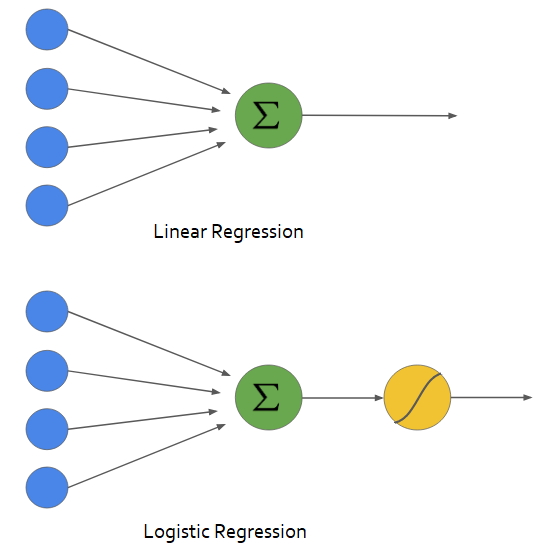
\includegraphics[width=2in]{figures/linearandlogistic}
\caption{Graphical representation of both linear and logistic regression.  The key difference is the application of the squashing function shown in yellow.  \href{https://towardsdatascience.com/building-a-logistic-regression-in-python-301d27367c24}{Original source}.}\label{fig:graphicaldataflow}
\end{marginfigure}
To make this intuition concrete, we define each $\hat{f}$ as having the following form (note: this equation looks daunting. We have some tips for interpreting it below).

\begin{align}
\hat{f}(\mathbf{x}) &= \mbox{probability that output, $y$, is 1} \nonumber \\
&=\frac{1}{1 + e^{-\mlvec{w}^\top \mathbf{x}}} \label{eq:logistichypothesis}
\end{align}

Here are a few things to notice about this equation:
\be
\item The weight vector that we saw in linear regression, $\mlvec{w}$, has made a comeback. We are using the dot product between $\mlvec{x}$ and $\mlvec{w}$ (which creates a weighted sum of the $x_i$'s), just as we did in linear regression!
\item As indicated in Figure~\ref{fig:graphicaldataflow}, the dot product $\mlvec{w}^\top \mlvec{x}$ has been passed through a squashing function known as the \href{https://en.wikipedia.org/wiki/Sigmoid_function}{sigmoid function}.  The graph of $\sigma(u) = \frac{1}{1+e^{-u}}$ is shown in Figure~\ref{fig:sigmoid}.  $\sigma( \mlvec{w}^\top \mlvec{x})$ is exactly what we have in Equation~\ref{eq:logistichypothesis}. 

\begin{marginfigure}
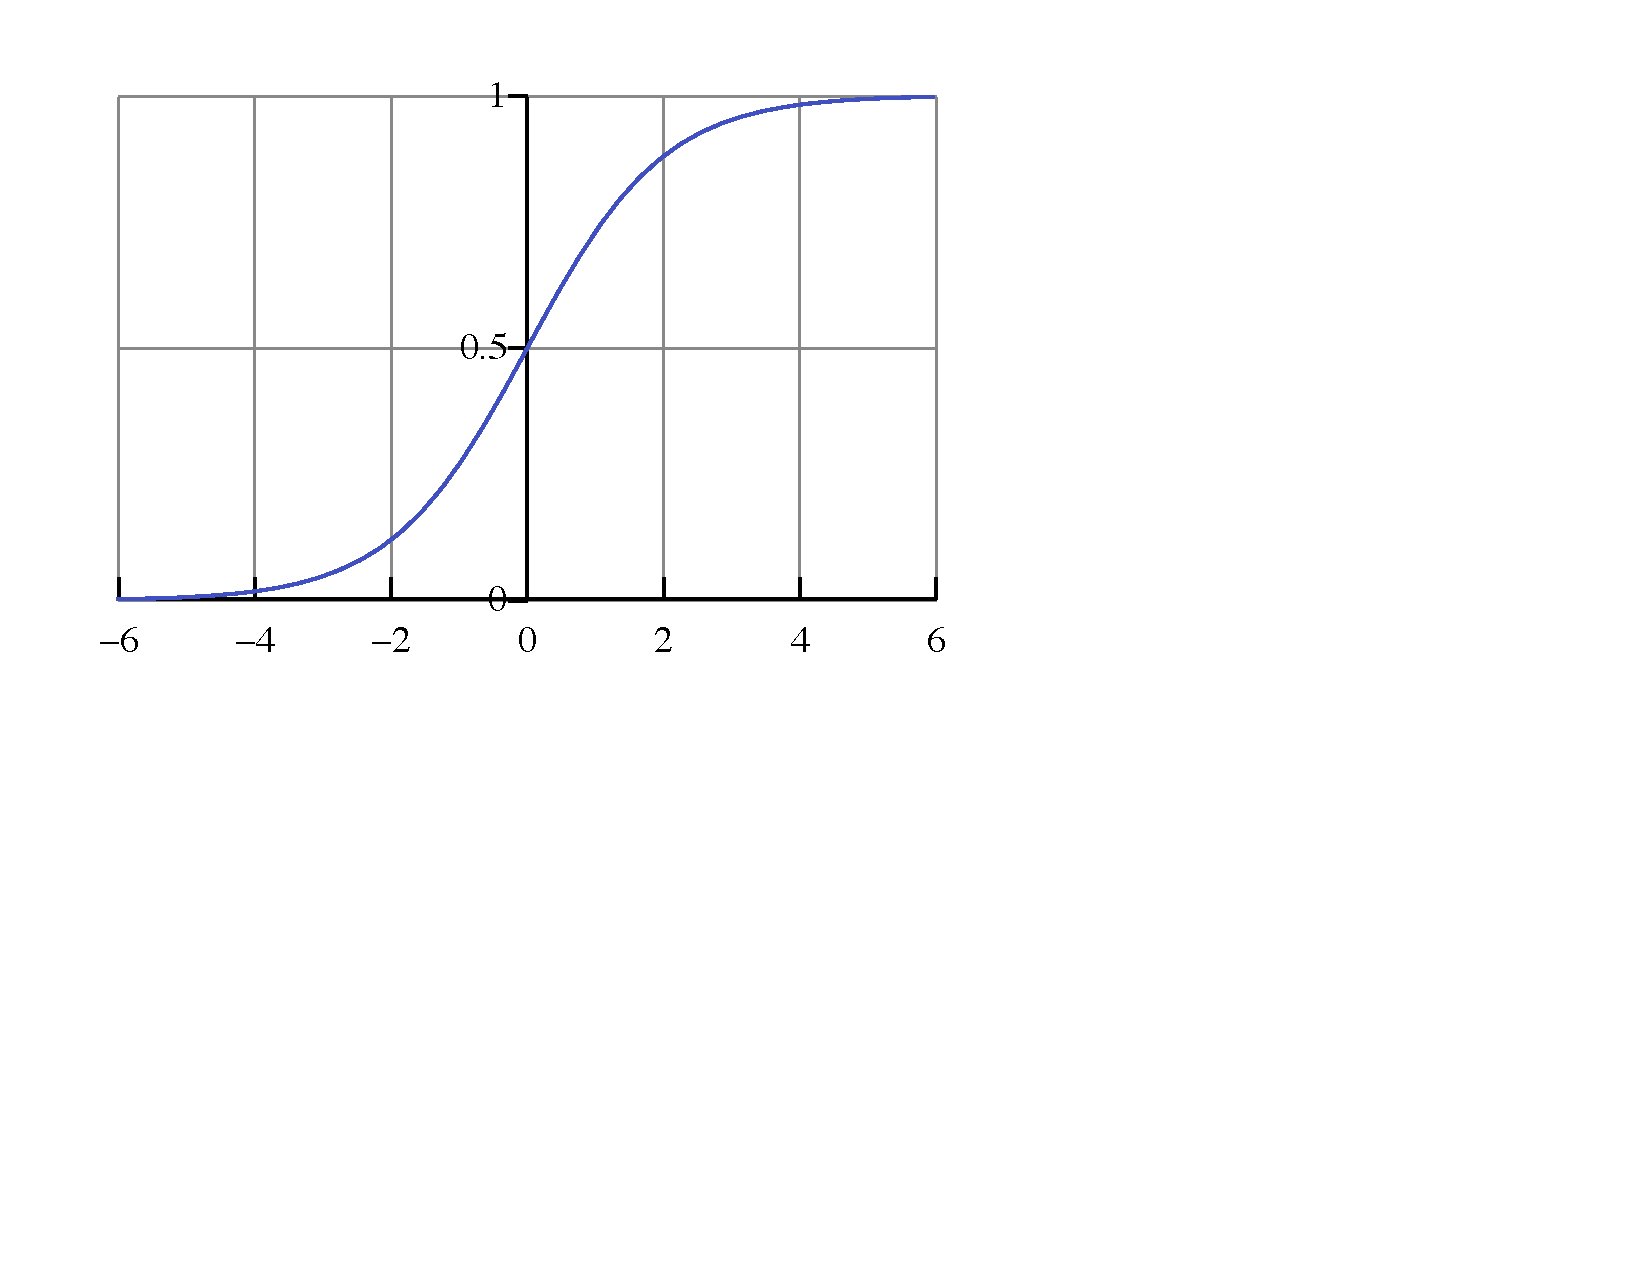
\includegraphics[width=\linewidth]{figures/Logistic-curve}
\caption{a graph of the sigmoid function $\frac{1}{1+e^{-x}}$.}\label{fig:sigmoid}
\end{marginfigure}
\ee

\subsection{Motivating Example: Sensor Networks}

\begin{notice}
Pretty much every writeup of logistic regression contains a simple two-independent variable example.  Usually these examples involve things like predicting who would be approved for a credit card or who will be admitted to a college.  We are going to do something a little messier and bit different.  If you want the admission to college example, you can read about it in \href{https://towardsdatascience.com/building-a-logistic-regression-in-python-301d27367c24}{Building a Logistic Regression in Python}.
\end{notice}

\begin{externalresources}[(60 minutes)]
Switch on over to the \href{https://colab.research.google.com/github/mlfa19/assignments/blob/master/Module\%201/03/Assignment_03_Companion.ipynb}{Assignment 3 Companion Notebook} for a presentation of the motivating example.
\end{externalresources}

\section{Putting it All Together: Deriving the Logistic Regression Learning Rule}
Let's summarize what we've done thus far in this assignment.

\bi
\item We motivated the binary classification problem.
\item We presented a particular useful loss function (log loss).
\item We met the logistic regression model and tried it out on a real dataset.
\ei

Next, we're going to build on these pieces and formalize the logistic regression problem and derive a learning rule to solve it (i.e., compute the optimal weights). The formalization of logistic regression will combine Equation~\ref{eq:logistichypothesis} with the selection of $\ell$ to be log loss.  This choice of $\ell$ results in the following objective function.

\begin{align}
\mlvec{w}^\star &= \argmin_{\mlvec{w}} \sum_{i=1}^n \left ( - y_i \ln \sigma(\mlvec{w}^\top \mlvec{x_i}) - (1-y_i) \ln (1 - \sigma(\mlvec{w}^\top \mlvec{x_i}) ) \right) \\
&= \argmin_{\mlvec{w}} \sum_{i=1}^n \left (  - y_i \ln \left ( \frac{1}{1+e^{-\mlvec{w}^\top \mlvec{x_i}}} \right) - (1-y_i) \ln  \left (1 - \frac{1}{1+e^{-\mlvec{w}^\top \mlvec{x_i}}} \right ) \right) &\mbox{expanded out if you prefer this form} \label{eq:objective}
\end{align}

While this looks a bit crazy, since $y_i$ is either 0 or 1, the multiplication of the expressions in the summation by either $y_i$ or $1-y_i$ are essentially acting like a switch---depending on the value of $y_i$ we either get one term or the other.  Our typical recipe for finding $\mlvec{w}^\star$ has been to take the gradient of the expression inside the $\argmin$, set it to $0$, and solve for $\mlvec{w}^\star$ (which will be a critical point and hopefully a minimum).  The last two steps will be a bit different for reasons that will become clear soon, but we will need to find the gradient.  We will focus on finding the gradient in the next couple of parts.

\subsection{Useful Properties of the Sigmoid Function}

Looking at Equation~\ref{eq:objective} it looks really, really hairy!  We see that in order to compute the gradient we will have to compute the gradient of $\mathbf{x}^\top \mlvec{w}$ with respect to $\mlvec{w}$ (we just wrapped our minds around this last assignment).  Additionally, we will have to take into account how the application of the sigmoid function and the log function changes this gradient.  In this section we'll learn some properties for manipulating the sigmoid function and computing its derivative.

\begin{exercise}[(60 minutes)]
The sigmoid function, $\sigma$, is defined as

\begin{align}
\sigma(x) &= \frac{1}{1+e^{-x}} \enspace .
\end{align}

\bes
\item Show that $\sigma(-x) = 1 - \sigma(x)$.
\begin{boxedsolution}
\begin{align}
\sigma(-x) &= \frac{1}{1+e^{x}} \\
&= \frac{e^{-x}}{e^{-x} + 1}~~\mbox{multiply by top and bottom by $e^{-x}$} \\
 \sigma(-x)  - 1&= \ \frac{e^{-x}}{e^{-x} + 1} - \frac{1 + e^{-x}}{1 + e^{-x}} ~~\mbox{subtract $-1$ on both sides} \\
 &= \frac{-1}{1+e^{-x}} \\
 &= -\sigma(x) \\
 \sigma(-x) &= 1 - \sigma(x)
\end{align}
\end{boxedsolution}
\item Show that the derivative of the logistic function $\frac{d}{dx} \sigma(x) = \sigma(x) (1 - \sigma(x))$

\begin{boxedsolution}
Two solutions for the price of 1!

Solution 1:
\begin{align}
\frac{d}{dx} \sigma(x)  &= -e^{-x} \sigma(x)^2 &\mbox{\href{https://www.math.hmc.edu/calculus/tutorials/quotient_rule/}{apply quotient rule}} \\
&= \sigma(x) \left ( \frac{-e^{-x}}{1 + e^{-x}} \right) &\mbox{expand out one of the $\sigma(x)$'s}\\
&= \sigma(x) \left ( \frac{-1}{e^{x} + 1} \right) & \mbox{multiply top and bottom by $e^{x}$}\\
&=  \sigma(x) ( - \sigma(-x)) &\mbox{substitute for $\sigma(-x)$} \\
&=  \sigma(x) ( \sigma(x) - 1) &\mbox{apply $\sigma(-x)=1-\sigma(x)$}
\end{align}

Solution 2:
\begin{align}
\frac{d}{dx} \sigma(x)  &=\frac{-e^{-x}}{(1+e^{-x} )^2} & \mbox{\href{https://www.math.hmc.edu/calculus/tutorials/quotient_rule/}{apply quotient rule}} \\
&= \frac{-e^{-x}}{1+2e^{-x} + e^{-2x}} & \mbox{expand the bottom}\\
&= \frac{-1}{e^{x}+2 + e^{-x}} & \mbox{multiply top and bottom by $e^{x}$}\\
&= \frac{-1}{(1+e^{x})(1+e^{-x})} & \mbox{factor} \\
&= -\sigma(x)\sigma(-x) & \mbox{decompose using definition of $\sigma(x)$}\\
&= -\sigma(x)(1-\sigma(x)) &\mbox{apply $\sigma(-x)=1-\sigma(x)$} \\
&= \sigma(x)(\sigma(x) - 1) & \mbox{distribute the $-1$}
\end{align}

\end{boxedsolution}
%
%\item \textbf{considering making this optional or just deleting} The log odds of an event occurring is defined as 
%\begin{align}
%\ln \left ( \frac{p(\mbox{event occurs})}{p(\mbox{event does not occur})} \right) = \ln \left ( \frac{p(\mbox{event occurs})}{1 - p(\mbox{event does occur})} \right) \enspace .
%\end{align}
%
%If we assume that $p(\mbox{event occurs}) = \sigma(x)$, show that the log odds of the event occurring is equal to $x$.
%
%\begin{boxedsolution}
%\begin{align}
%\ln \left ( \frac{p(\mbox{event occurs})}{p(\mbox{event does not occur})} \right)  &= \ln \left ( \frac{\sigma(x)}{1 - \sigma(x)} \right ) \\
%&= \ln \left ( \frac{\sigma(x)}{\sigma(-x)} \right ) \\
%&= \ln \left ( \frac{1 + e^x}{1+e^{-x}} \right) \\
%&= \ln \left ( e^x \frac{1 + e^x}{e^{x}(1+e^{-x})} \right) \\
%&= x + \ln \left ( \frac{1+e^x}{e^{x} + 1} \right) \\
%&= x
%\end{align}
%\end{boxedsolution}

\ees

\end{exercise}

\subsection{Chain Rule for Gradients}
We now know how to take derivatives of each of the major pieces of Equation~\ref{eq:objective}.  What we need is a way to put these derivatives together.  You probably remember that in the case of single variable calculus you have just such a tool.  This tool is known as the chain rule.  The chain rule tells us how to compute the derivative of the composition of two single variable functions $f$ and $g$.  

\begin{align}
h(x)&= g(f(x))&\mbox{h(x) is the composition of $f$ with $g$} \nonumber \\
h'(x) &= g'(f(x))f'(x)&\mbox{this is the chain rule!}
\end{align}

Suppose that instead of the input being a scalar $x$, the input is now a vector, $\mlvec{w}$.  In this case $h$ takes a vector input and returns a scalar, $f$ takes a vector input and returns a scalar, and $g$ takes a scalar input and returns a scalar.

\begin{align}
h(\mlvec{w}) &= g(f(\mlvec{w}))&\mbox{h($\mlvec{w}$) is the composition of $f$ with $g$} \nonumber \\
\nabla h(\mlvec{w}) &= g'(f(\mlvec{w})) \nabla f(\mlvec{w}) & \mbox{this is the multivariable chain rule}
\end{align}

\begin{exercise}[(60 minutes)]
\bes
\item Suppose $h(x) = \sin(x^2)$, compute $h'(x)$ (x is a scalar so you can apply the single-variable chain rule).

\begin{boxedsolution}

Applying the chain rule gives
\begin{align}
h'(x) &= cos(x^2) 2x \enspace .
\end{align}
\end{boxedsolution}

\item Define $h(\mlvec{v}) = (\mlvec{c}^\top \mlvec{v})^2$.  Compute $\nabla_{\mlvec{v}} h(\mlvec{v})$ (the gradient of the function with respect to $\mlvec{v}$).

\begin{boxedsolution}
We can see that $h(\mlvec{v}) = g(f(\mlvec{v}))$ with $g(x) = x^2$ and $f(\mlvec{v}) = \mlvec{c}^\top \mlvec{v}$ The gradient can now easily be found by applying the chain rule.
\begin{align}
\nabla h(\mlvec{v}) &= 2(\mlvec{c}^\top \mlvec{v}) \mlvec{c}
\end{align}
\end{boxedsolution}

\item Compute the gradient of the expression from Equation~\ref{eq:objective} (reproduced below for your convenience).

\begin{align}
 \sum_{i=1}^n -y_i \ln \sigma( \mlvec{w}^\top \mlvec{x_i}) - (1-y_i) \ln  \left (1 - \sigma( \mlvec{w}^\top \mlvec{x_i}) \right ) \enspace .
\end{align}

You can either use the chain rule and the identities you learned about sigmoid, or expand everything out and work from that.

\begin{boxedsolution}
Applying the chain rule gives us

\begin{align}
 \sum_{i=1}^n -y_i \frac{\nabla \sigma( \mlvec{w}^\top \mlvec{x_i})}{\sigma( \mlvec{w}^\top \mlvec{x_i})} - (1-y_i) \frac{- \nabla \sigma( \mlvec{w}^\top \mlvec{x_i})}{1 - \sigma( \mlvec{w}^\top \mlvec{x_i})}  \enspace .
\end{align}

Applying the chain rule again gives us
\begin{align}
& \sum_{i=1}^n -y_i \frac{\sigma( \mlvec{w}^\top \mlvec{x_i})(1-\sigma( \mlvec{w}^\top \mlvec{x_i}))\nabla \mlvec{w}^\top \mlvec{x_i}}{\sigma( \mlvec{w}^\top \mlvec{x_i})} - (1-y_i) \frac{- \sigma( \mlvec{w}^\top \mlvec{x_i})(1-\sigma( \mlvec{w}^\top \mlvec{x_i}))\nabla \mlvec{w}^\top \mlvec{x_i}}{1 - \sigma( \mlvec{w}^\top \mlvec{x_i})} \nonumber \\
 &= \sum_{i=1}^n -y_i (1-\sigma( \mlvec{w}^\top \mlvec{x_i}))\mlvec{x_i} + (1-y_i)  \sigma( \mlvec{w}^\top \mlvec{x_i})) \mlvec{x_i} 
 \end{align}
 
You could certainly stop here, but if you plug in $y=0$ and $y=1$ you'll find that the expression can be further simplified to:
 
 \begin{align}
\sum_{i=1}^n  -(y_i - \sigma(\mlvec{w}^\top \mlvec{x_i})) \mlvec{x_i} \nonumber
 \end{align}


\end{boxedsolution}

\ees
\end{exercise}


\subsection{Gradient Descent for Optimization}
If we were to follow our derivation of linear regression we would set our expression for the gradient to 0 and solve for $\mlvec{w}$.  It turns out this equation will be difficult to solve due to the $\sigma$ function.  Instead, we can use an iterative approach where we start with some initial value for $\mlvec{w}$ (we'll call the initial value $\mlvec{w^0}$, where the superscript corresponds to the iteration number) and iteratively adjust it by moving down the gradient (the gradient represents the direction of fastest increase for our function, therefore, moving along the negative gradient is the direction where the loss is decreasing the fastest).

\vspace{1em}
\begin{externalresources}[(45 minutes)]
There are tons of great resources that explain gradient descent with both math and compelling visuals.
\bi
\item Recommended: \href{https://www.youtube.com/watch?v=IHZwWFHWa-w}{Gradient descent, how neural networks learn | Deep learning, chapter 2} (start at 5:20)
\item An Introduction to Gradient Descent (\href{http://nb.mit.edu/f/55231}{on NB}, \href{https://medium.com/@viveksingh.heritage/an-introduction-to-gradient-descent-54775b55ba4f}{original})
\item The Wikipedia page on Gradient Descent (\href{http://nb.mit.edu/f/55232}{on NB}, \href{https://en.wikipedia.org/wiki/Gradient_descent}{original})
\item \href{https://www.youtube.com/watch?v=fPSPdTjINi0}{Ahmet Sacan's video on gradient descent} (this one has some extra stuff, but it's pretty clearly explained).
\item There are quite a few resources out there, do you have some suggestions? (suggest so on NB)
\ei 
\end{externalresources}

\begin{exercise}[(10 minutes)]
To test your understanding of these resources, here are a few diagnostic questions.
\bes
\item When minimizing a function with gradient descent, which direction should you step along in order to arrive at the next value for your parameters?
\begin{boxedsolution}
The negative gradient (since we are minimizing)
\end{boxedsolution}

\item What is the learning rate and what role does it serve in gradient descent?
\begin{boxedsolution}
The learning rate controls the size of the step that you take along the negative gradient.
\end{boxedsolution}

\item How do you know when an optimization performed using gradient descent has converged?
\begin{boxedsolution}
There are a few options.  One popular one is to check if the objective function is changing only only a minimal amount each iteration, the algorithm has converged.  You could also look at the magnitude of the gradient (which tells us the slope) to see if it is really small.
\end{boxedsolution}

\item True or false: provided you tune the learning rate properly, gradient descent guarantees that you will find the global minimum of a function.
\begin{boxedsolution}
False, the best gradient descent can do, in general, is converge to a local minimum.  If you know that the function you are optimizing has only one minimum, then this would also be the global minimum (this is the case for both linear and logistic regression).
\end{boxedsolution}
\ees
\end{exercise}

If we take the logic of gradient descent and apply it to the logistic regression problem, we arrive at the following learning rule.  Given some initial weights $\mlvec{w^0}$, and a learning rate $\eta$, we can iteratively update our weights using the formula below.

\begin{align}
\mlvec{w^{n+1}} &= \mlvec{w^n} - \eta \sum_{i=1}^n  -(y_i - \sigma(\mlvec{w}^\top \mlvec{x_i})) \mlvec{x_i} ~~~\mbox{applying the result from exercise 4} \\
&=  \mlvec{w^n} + \eta \sum_{i=1}^n  (y_i - \sigma(\mlvec{w}^\top \mlvec{x_i})) \mlvec{x_i}  ~~~\mbox{distribute the negative}
\end{align}

This beautiful equation turns out to be the recipe we need to implement logistic regression.

\begin{exercise}[\faShareAlt~(10 minutes)]
Now that you've had a second round of working with an in-class partner, we want to hear more about how it's going.
\bes
\item Did you and your partner work well together?  To help us understand how this better, provide a concrete examples to illustrate what went well and what didn't.  If you want to avoid working with you partner in the future, say so (make sure to include the person's name).  Only use this option in extenuating circumstances.
\item We are assigning partners as an experiment.  Our rationale for this choice is that finding a partner is potentially stressful and it may be difficult to work with folks you don't normally socialize with.  With this rationale in mind, do you think we should continue to assign class work partners?  Should we tweak this somehow?
\ees
\end{exercise}

%
%
%
%\section{Reading on TODO}
%TODO
%
%\section{Suggestions for Additional Challenge (NOTE: I'm on the fence about these.  What do you think?}
%
%We are asking folks for whom this is review to push themselves a bit farther.  Based on the first two assignments, we thought that we could help out with some suggestions of our own.  Please don't construe this as work that you have to do.  None of the course content will assume that you've done any of these additional activities.
%
%\begin{itemize}
%\item Implement logistic regression using gradient descent.  You will need to search for a good learning rate or you may consider implementing some \href{https://towardsdatascience.com/gradient-descent-algorithms-and-adaptive-learning-rate-adjustment-methods-79c701b086be}{strategies for automatically tuning the learning rate}.
%\item Some additional reading?
%\end{itemize}

\companionnotebook{Assignment_03_Companion}


\end{document}
